\section{Αμφιωτικές Παράμετροι} \label{sec:binaural_cues}


Το ακουστικό σύστημα, μπορεί να παρομοιαστεί με έναν υπολογιστή πολλαπλών χρήσεων με δύο θύρες εισόδου. Οι θύρες είναι τα δύο αυτιά, στο ίδιο ύψος εκατέρωθεν ενός στερεού ελλειψοειδούς, το κεφάλι.  Το κεφάλι λειτουργεί ως \textit{φορέας μιας κεραίας}, που μπορεί να κινηθεί με έξι βαθμούς ελευθερίας σε σχέση με το σώμα, ενώ το ίδιο το σώμα μπορεί να προηγηθεί στον τρισδιάστατο χώρο, και να αλλάξει τον προσανατολισμό του σε σχέση με τη θέση αναφοράς \cite{Kohlrausch2013}. Μία σύντομη ανατομική περιγραφή του ακουστικού συστήματος φαίνεται στο Σχήμα \ref{fig:auditory_system}

\begin{figure}[h]
  \centering
  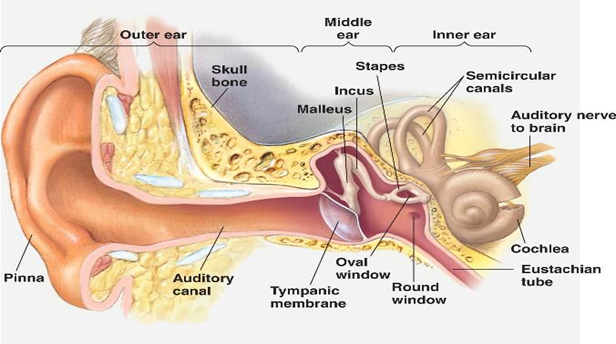
\includegraphics[width=\textwidth]{images/auditory_system.png}
  \caption{Ανατομική περιγραφή του ακουστικού συστήματος}
  \label{fig:auditory_system}
\end{figure}

Το ακουστικό σύστημα δέχεται εισόδους με τη μορφή ελαστικών δονήσεων και κυμάτων, από υγρά ή στερεά με τα οποία είναι σε μηχανική επαφή. Οι είσοδοι έρχονται είτε μέσω του αέρα από τα ακουστικά κανάλια (ear canals) είτε από την μεταβίβαση των οστών μέσω του κρανίου. Συνήθως το κρανίο αγνοείται όταν πρόκειται για ακρόαση σε αέρα, αφού διαφέρει κατά περίπου 60 dB σε σχέση με την μεταβίβαση λόγω αέρα, που αντιστοιχεί σε έναν λόγο ισχύος της τάξεως του $10^6$.

Η ακοή επιτυγχάνεται και με ένα μόνο αυτί, αλλά η ακρόαση με δύο λειτουργικά αυτιά, ή \textit{αμφιωτική ακρόαση}, προσφέρει σημαντικά πλεονεκτήματα έναντι της μονοωτικής ακρόασης. Αυτό, συμβαίνει διότι η αμφιωτική ακρόαση προσφέρει επιπλέον πληροφορία, η οποία κωδικοποιείται στις διαφορές των σημάτων εισόδου στα δύο αυτιά.

Υποθέτοντας ότι αυτές οι διαφορές αναπαρίστανται με ένα γραμμικό, χρονικά αμετάβλητο σύστημα, προκύπτει το συμπέρασμα, ότι μπορούν να υπάρχουν μόνο δύο τέτοιες διαφορές. Η αμφιωτική διαφορά χρόνου άφιξης (Interaural Time Difference - ITD) και οι αμφιωτικές διαφορές έντασης (Interaural Level Difference - ILD). Και οι δύο εξαρτώνται από τη συχνότητα.

Τα υπάρχοντα μοντέλα, αξιοποιούν τις ακουστικές παραμέτρους, που διακρίνονται σε αμφιωτικές παραμέτρους, που είναι πιο εύρωστες και απαιτούν και τα δύο αυτιά για να αναλυθούν, και σε μονοωτικές παραμέτρους που χρειάζονται μόνο το ένα αυτί. Εδώ αναλύονται μόνο οι αμφιωτικές παράμετροι αφού αυτές χρησιμοποιήθηκαν για την προσέγγιση του προβλήματος.

\subsection{Interaural Time Difference}

Παρουσιάζεται πρώτα η ανάλυση του ITD, γιατί ιστορικά το μοντέλο Jefress \cite{Jeffress1948} ήταν το πρώτο μοντέλο εντοπισμού, το 1948. Η βασική ιδέα αυτού του μοντέλου είναι ένας συνδυασμός, \textit{γραμμών καθυστέρησης} και \textit{κυττάρων σύμπτωσης} (coincidence cells). Με βάση το μοντέλο, υπάρχουν δύο ξεχωριστές, παράλληλες γραμμές καθυστέρησης σε κάθε αυτί. Τα σήματα διαδίδονται με αντίθετη κατεύθυνση σε κάθε γραμμή, όπως φαίνεται στο Σχήμα \ref{fig:jeffress-coincidence-mechanism}. Σε κάποιο σημείο, τα σήματα που ταξιδεύουν στις δύο γραμμές, συναντούνται σε ένα κύτταρο σύμπτωσης, το οποίο στέλνει το σήμα στο επόμενο επίπεδο. Λόγω της διαφοράς χρόνου άφιξης των δύο σημάτων στα αυτιά, αυτά θα ενεργοποιήσουν ένα πλευρικά μετατοπισμένο κύτταρο σύμπτωσης, το οποίο κατ' επέκταση αντιστοιχίζεται σε μια πλευρική γωνία άφιξης.

Οι Cherry και Sayers \cite{Cherry1956}, εισήγαγαν τη χρήση της αμφιωτικής ετεροσυσχέτισης, ως μια μέθοδο για την εκτίμηση του ITD η οποία ορίζεται όπως φαίνεται στην Εξίσωση \ref{IACC}. Με την εσωτερική καθυστέρηση να ορίζεται με \textit{τ} και τα αριστερά και δεξιά σήματα πίεσης, $y_l(t)$ και $y_r(t)$. Έχει αποδειχτεί πως αυτό είναι μια καλή προσέγγιση του μοντέλου Jeffress. Το ITD έχει παρατηρηθεί πως δεν παίζει ιδιαίτερο ρόλο στον εντοπισμό πηγών σε συχνότητες μεγαλύτερες των 1500Hz.

\begin{CEquation}
    \psi_{y_{l,r}}(\tau) = \frac{\int_{t=-\infty}^{\infty}y_l(t)y_r(t+\tau)dt}
    {\sqrt{\int_{t=-\infty}^{\infty}y_l^2(t)dt \int_{t=-\infty}^{\infty}y_r^2(t)dt}}
    \label{IACC}
\end{CEquation}

\begin{figure}[h]
  \centering
  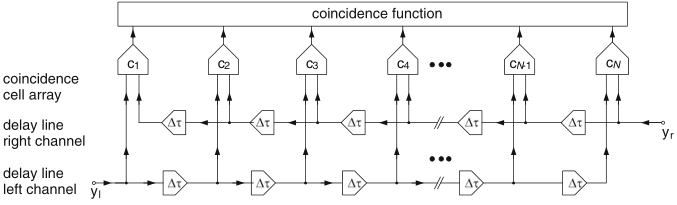
\includegraphics[width=\textwidth]{images/jeffress-coincidence-mechanism.png}
  \caption{Μοντέλο σύμπτωσης όπως αρχικά προτάθηκε από τον Jeffress}
  \label{fig:jeffress-coincidence-mechanism}
\end{figure}

\subsection{Interaural Level Difference}

Οι αμφιωτικές διαφορές έντασης συμβαίνουν λόγω φαινομένων επικάλυψης του κεφαλιού, όταν ένας ήχος φτάνει πλάγια στον δέκτη. Τυπικές τιμές είναι $\pm30 dB$ σε συχνότητες κοντά στα 5 kHz και γωνίες άφιξης στα $\pm60^o$. Στις χαμηλές συχνότητες η επικάλυψη του κεφαλιού δεν παίζει ιδιαίτερο ρόλο, και διαφορές στο ILD σπανίζουν (κάτω από 1500 Hz). Η συχνότητα επικάλυψης ILD και ITD γίνεται φανερό πως είναι στα 1500 Hz.

Το ILD, μπορεί να υπολογιστεί απευθείας από τα σήματα του αριστερού και δεξιού καναλιού όπως φαίνεται στην εξίσωση \ref{ILD_1}, πράγμα το οποίο τυπικά υπολογίζεται για διαφορετικές μπάντες συχνοτήτων, όπου $P_l$ και $P_r$ οι ισχύες των σημάτων που φτάνουν στο αριστερό και δεξί αυτί.
\begin{CEquation}
    \alpha = 10log_{10}(P_l) - 10log_{10}(P_r)
    \label{ILD_1}
\end{CEquation}
Οι Reed και Blum \cite{Reed1990} εισήγαγαν έναν φυσιολογικό (physiological) αλγόριθμο για τον υπολογισμό του ILD, βασισμένο στην δραστηριότητα, $E(\alpha)$, μιας συστοιχίας \textit{El cells}, όπως φαίνεται στο σχήμα \ref{fig:el-cell-structure} και περιγράφεται στην Εξίσωση \ref{eq:reed-and-blum}. Η απόκριση κάθε El-cell είναι συντονισμένη για ένα συγκεκριμένο ILD, και ελατώνεται όσο πιο μακριά από αυτό είναι το ILD των σημάτων άφιξης.

\begin{CEquation}
    E(\alpha) = \exp{
    (10^{\alpha \slash ILD_{max}}\sqrt{P_l} - 
    10^{\alpha \slash ILD_{max}}\sqrt{P_r}})^2
    \label{eq:reed-and-blum}
\end{CEquation}

\begin{figure}[h]
  \centering
  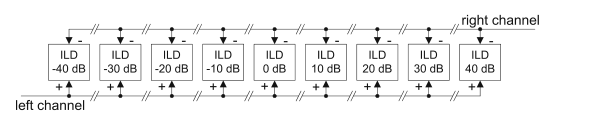
\includegraphics[width=\textwidth]{images/el-cell-structure.png}
  \caption{Δομή El-cell}
  \label{fig:el-cell-structure}
\end{figure}

\subsection{Εντοπισμός ηχητικών γεγονότων}

Υπάρχουν πολλές μέθοδοι για τον υπολογισμό της θέσης ηχητικών πηγών από τις αμφιωτικές παραμέτρους. Μια μέθοδος που επιτυγχάνει αυτόν τον σκοπό, είναι η κατασκευή μια βάσης δεδομένων, που αντιστοιχίζει μετρηθείσες παραμέτρους ILD και ITD σε σφαιρικές συντεταγμένες.

Είναι ακόμα ασαφές πως το ακουστικό σύστημα συνδυάζει τις παραμέτρους για την εξαγωγή συμπερασμάτων για την θέση ακουστικών γεγονότων, συγκεκριμένα, αναπάντητα είναι ακόμα τα εξής ερωτήματα:


\begin{itemize}
    \item Ο τρόπος που συνδυάζονται τα ILD και ITD.
    \item Η ολοκλήρωση της πληροφορίας ως προς τον χρόνο.
    \item Η ολοκλήρωση της πληροφορίας ως προς τη συχνότητα.
    \item Ο διαχωρισμός διαφορετικών, ταυτόχρονων πηγών.
    \item Η αντιμετώπιση των ανακλάσεων του δωματίου.
\end{itemize}

Ότι είναι γνωστό μέχρι στιγμής για τον τρόπο που το ακουστικό σύστημα συνδυάζει τις παραμέτρους έχει προκύψει πειραματικά, από τα αποκαλούμενα trading πειράματα, όπου το ILD υποδεικνύει μια κατεύθυνση, αλλά το ITD μια διαφορετική και ο δέκτης καλείται να κρίνει την πραγματική.

Πιστεύεται ότι το ακουστικό σύστημα, εφαρμόζει χρονικό ή/και συχνοτικό cue weighting, δηλαδή δίνει μεγαλύτερη βαρύτητα σε κάποιες παραμέτρους όταν πληρούνται κάποιες συνθήκες, αλλά ο ακριβής τρόπος που αυτό συμβαίνει είναι ακόμα υπό διερεύνηση. Υπάρχουν διαφορετικές απόψεις, με την μία, που είναι και η επικρατέστερη, να λέει πως το ακουστικό σύστημα δίνει έμφαση στο onset τμήμα του σήματος, ενώ η άλλη να ισχυρίζεται πως ολοκληρώνει την πληροφορία σε μεγαλύτερο χρονικό διάστημα. Τα πράγματα γίνονται σημαντικά δυσκολότερα, όταν δεν είναι σαφές πόσες πηγές υπάρχουν. Τότε οι παράμετροι εκτός από την ανάθεση βαρών σε αυτές, πρέπει να αντιστοιχηθούν και στη σωστή πηγή. Η μεγαλύτερη πρόκληση όμως παραμένει διερεύνηση της αντιμετώπισης των ανακλάσεων του δωματίου από το ακουστικό σύστημα.